\documentclass[twoside,twocolumn]{article}

\usepackage{blindtext} 
\usepackage{graphicx}
\usepackage[sc]{mathpazo} 
\usepackage[T1]{fontenc} 
\linespread{1.05} 
\usepackage{microtype} 


\usepackage[english]{babel} 


\usepackage[hmarginratio=1:1,top=32mm,columnsep=20pt]{geometry} 
\usepackage[hang, small,labelfont=bf,up,textfont=it,up]{caption} 
\usepackage{booktabs} 


\usepackage{lettrine} 


\usepackage{enumitem} 
\setlist[itemize]{noitemsep} 


\usepackage{abstract} 
\renewcommand{\abstractnamefont}{\normalfont\bfseries} 
\renewcommand{\abstracttextfont}{\normalfont\small\itshape} 


\usepackage{titlesec} 
\renewcommand\thesection{\Roman{section}} % 
\renewcommand\thesubsubsection{\roman{subsubsection}} 
\titleformat{\section}[block]{\large\scshape\centering}{\thesection.}{1em}{} 
\titleformat{\subsubsection}[block]{\large}{\thesubsubsection.}{1em}{} 


\usepackage{fancyhdr} 
\pagestyle{fancy} % All pages have headers and footers
\fancyhead{} % Blank out the default header
\fancyfoot{} % Blank out the default footer
\fancyhead[L]{Analítica de Negocios vs Inteligencia de Negocios} % Custom header text
\fancyhead[R]{March 2021} % Custom header text
\fancyfoot[RO,LE]{\thepage} % Custom footer text


\usepackage{titling} 


\usepackage{hyperref} 


%----------------------------------------------------------------------------------------
%	TILULOS
%----------------------------------------------------------------------------------------

\setlength{\droptitle}{-4\baselineskip} 

\pretitle{\begin{center}\Huge\bfseries} 
\posttitle{\end{center}} 
\title{Analítica de Negocios vs Inteligencia de Negocios} 
\author{Jose Arias, Jose Gutierrez, Posi Vargas, Rodrigo Yanqui, Roby Zuñiga}
\date{\today} 
\renewcommand{\maketitlehookd}{
\begin{abstract}
\noindent
    ¿Cuál es la diferencia Analista de Datos (BA) e Inteligencia de negocios (BI)?.Esta es una pregunta que se estado hablando mucho, lo he recibido personalmente de un puñado de personas.
    En este artículo escribiremos sobre la diferencia entre Analista de Datos (BA) e Inteligencia de negocios (BI). Algunos dicen que BI es el análisis de situaciones pasadas y BA el trata de predecir el futuro con la data. Algunos dicen que BI es el análisis de situaciones pasadas y BA el tratar de predecir el futuro con la data.
\end{abstract}
\begin{abstract}
\noindent 
    What is the data analyst difference (BA) and business intelligence (BI)? This is a question that was speaking a lot, I have personally received it from a handful of people.
    In this article we will write about the difference between data analyst (BA) and business intelligence (BI). Some say that BI is the analysis of past situations and BA TRAWS TO PREDIVE THE FUTURE WITH THE DATA. Some say that BI is the analysis of past situations and to try to predict the future with the data.
\end{abstract}
}

%----------------------------------------------------------------------------------------

\begin{document}

% Print the title
\maketitle

%----------------------------------------------------------------------------------------
%	INTRODUCCION
%----------------------------------------------------------------------------------------

\section{Introduccion}
\lettrine[nindent=0em,lines=3]{E}n los últimos años muchas compañías se han percatado de las posibilidades que ofrece el Big Data, y están optando por integrar tanto el BI como el BA bajo un mismo departamento operacional. De cara al cliente, la inmediatez de los beneficios que ofrece el Business Intelligence está provocando que tome ventaja respecto a su técnica homóloga.\\ \\
Cada una de ellas tiene un objetivo distinto. La Inteligencia Empresarial analiza datos para ofrecer soluciones que permitan optimizar las actividades presentes, mientras que la Analítica Empresarial analiza datos para anticipar peligros y posibilidades futuras.\\ \\
Para saber cuál es la adecuada para tu negocio debes tener en cuenta dos variables: tamaño e intención. Antiguamente el BI era más común en las grandes compañías, pero en los últimos años la tendencia apunta hacia las pymes, y hacia el Self-service Business Intelligence (SSBI); un enfoque que permite funcionar a empresas sin recorrido en el campo del Big Data. \\ \\
Aquella empresa que si lleva a cabo procesos de extraccion de datos, transformacion de datos, uso de herramientas y metodos, tendra una ventaja notoria a comparacion de las demas que no lo aplican.\\ \\
Si lo que se busca es mejorar y optimizar resultados, quizás la mejor opción es el Business Intelligence. Por el contrario, si se piensa en emprender un cambio de rumbo, será mejor prever riesgos con el Business Analytics. Siempre teniendo en cuenta la formación de los empleados.

%----------------------------------------------------------------------------------------
%	DESARROLLO
%----------------------------------------------------------------------------------------

\section{Desarrollo}

\subsection{INTELIGENCIA DE NEGOCIOS}
La Inteligencia de Negocios es un conjunto de estrategias, tecnologías, aplicaciones enfocadas a la administración y creación de conocimiento sobre nuestro negocio, a través del análisis de datos de una organización o empresa. De una manera más concreta, es la habilidad para transformar los datos en información, y la información en conocimiento, de forma que se pueda optimizar el proceso de toma de decisiones en los negocios.

\subsection{COMPONENTES DE LA INTELIGENCIA DE NEGOCIOS}
\begin{itemize}
    \item  Minería de Datos
    \item  Administración del Conocimiento
    \item  Aplicaciones Analíticas
    \item  Sistemas de Reportes
    \item  Multidimensionalidad
    \item  Data Warehouse   
\end{itemize}

\subsection{ETAPAS DE INTELIGENCIA DE NEGOCIOS}
\subsubsection{Etapa de extracción}
El proceso de implementación de un sistema de inteligencia de negocios en una organización debe iniciar por seleccionar la información relevante para la toma de decisiones, esto requiere contar con la participación de personal en los niveles operativo, táctico y gerencial.
\subsubsection{Etapa de consolidación}
Esta etapa consiste de la recopilación de los datos de las diferentes fuentes, ya sean internas o externas de manera automática o semiautomática con el fin de normalizarlos, depurarlos y estructurarlos, almacenándolos en la bodega de datos, todo ello teniendo en cuenta que se debió haber hecho un análisis exhaustivo de las necesidades de información de la organización (etapa previa).
\subsubsection{Etapa de explotación}
En ésta etapa es donde se comienzan a aplicar las herramientas existentes para dejar listos los datos de la bodega en manos de los usuarios, quienes deben estar en capacidad de empezar a aprovechar y explotar la información ya depurada y filtrada que hay en la bodega de datos. 
\subsubsection{Etapa de visualización}
Después de realizar la explotación, continua una etapa de visualización, donde los usuarios a través de ciertas herramientas gráficas pueden conocer de primera mano lo que está sucediendo en la organización, esta etapa involucra las siguientes metodologías y/o herramientas: Balance Scored Card, Sistemas de Soporte a la Decisión (DSS), Sistemas de Información Ejecutiva (EIS).
\subsubsection{Análisis del mercado}
Las principales empresas del sector Business Intelligence son:
\begin{itemize}
    \item Microsoft 
    \item Oracle 
    \item Microstrategy 
    \item IBM Cognos 
    \item Information Builders 
    \item SAS 
    \item QlikTech 
    \item SAP Business Objects 
    \item Teradata 
    \item Hyperion 
    \item Tableau 
    \item Netezza 
    \item Pentaho
\end{itemize}

\subsection{¿POR QUÉ ES IMPORTANTE EL BUSINESS INTELLIGENCE?}
Porque nos ayuda a tomar esa data y vamos a desplegarla de una forma, donde el tomador de decisiones pueda saber exactamente lo que debe de hacer, claro eso va a depender de la persona que está tomando las decisiones, pero la esencia de la inteligencia de negocios, es facilitar la toma de decisiones.\\ \\
\begin{center}
    \textit{Es importante resaltar que no estamos dejando afuera la parte predictiva, debemos saber cómo hacer predicciones, pero nos vamos a enfocar más que todo, en la parte de despliegue.}
\end{center}

\subsection{ARQUITECTURA DE INTELIGENCIA DE NEGOCIO}
Arquitectura típica genérica que acompaña un modelo de inteligencia de negocios a través del cual, aprovechando las bondades que nos ofrece la tecnología, es posible disponer de información cuantitativa oportuna y de calidad para la toma de decisiones institucionales.
\begin{center}
    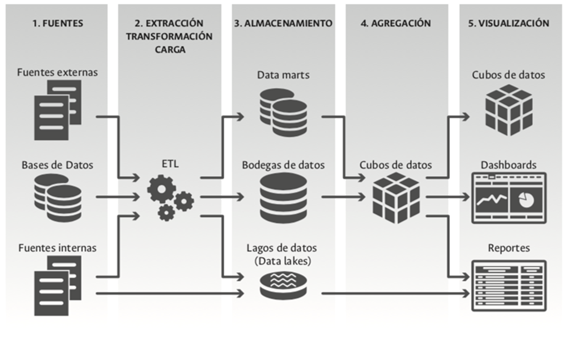
\includegraphics[width=7cm]{./img/img1.png} 
\end{center}

\subsection{HERRAMIENTAS PARA HACER INTELIGENCIA DE NEGOCIOS}
En el contexto contemporáneo, cuando hablamos de Inteligencia de Negocios, asumimos que la tecnología juega un rol vital. Podríamos hacer “Business Intelligence” con papel y lápiz, o simplemente usando MSExcel, pero en la actualidad se han desarrollado muchas herramientas tecnológicas para hacer que el análisis de un negocio sea más fácil. La tecnología nos apoya con:
\begin{enumerate}
    \item Colectar la información. 
    \item Guardar esa información y 
    \item Poder hacer algo con esa información 
\end{enumerate}
Hoy por hoy existen un sinfín de herramientas y software para realizar Inteligencia de Negocios,
\begin{itemize}
    \item Domo
    \item Tableou
    \item Power BI
    \item SaS
\end{itemize}
\begin{center}
    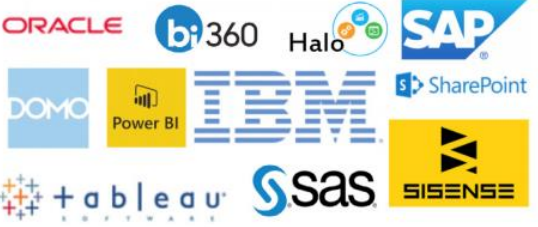
\includegraphics[width=7cm]{./img/img2.png} 
\end{center}

\subsection{ANALÍTICA DE NOGOCIOS}
La Analítica de negocios o business analytics comprende el conjunto de métodos de análisis básicos que conlleva el uso de datos para conocer qué ha pasado o qué está pasando en este momento (descriptivo), así como métodos de análisis avanzados para saber qué pasará (predictivo) o qué debería suceder en el futuro (prescriptivo).\\ \\
En otros términos, la analítica de negocio consiste en crear conocimiento de valor a partir del análisis de datos masivos con el propósito de extraer patrones de comportamiento sobre nuestros hábitos y costumbres, así como interpretar de forma eficiente situaciones empresariales para tomar decisiones informadas e inteligentes.

\subsection{POR QUÉ ES IMPORTANTE EL BUSINESS ANALYTICS}
Según el artículo "Analítica de negocios: ¿qué es y por qué es importante?" de Harvard Business Review, existen tres razones por las que una empresa debería tener en cuenta la importancia de Business Analytics.
\begin{enumerate}
    \item Permite tomar decisiones más informadas
    \item Ayuda a generar más ingresos
    \item Logra mejorar las operaciones comerciales
\end{enumerate}

\subsection{HERRAMIENTAS DE BUSINESS ANALYTICS}
Para ayudar a los analistas a procesar la información y poder generar propuestas de mejora, la analítica de negocios cuenta con muchas metodologías y software especializados en encontrar soluciones. Según MicroStrategy, estas son algunas de las herramientas de Business Analytics más populares -y potentes- del momento.
\begin{itemize}
    \item Birt
    \item Apache Zeppelin
    \item OmniSci
    \item SpagoBI
    \item Matomo Analytics
    \item Metabase
\end{itemize}

\subsection{ETAPAS DE BUSINESS ANALYTICS}
\subsubsection{Análisis descriptivo: ¿Qué pasó?}
La primera etapa del Analytics Lifecycle consta del análisis descriptivo, que permite comprender qué pasó y qué está pasando en el negocio actualmente, al procesar los datos en crudo y transformarlos en información que los usuarios puedan comprender y utilizar para comprender la situación en el que se encuentra la empresa y tener un contexto válido sobre el que preparar acciones futuras. Para hacer este análisis las empresas se valen de soluciones de Business Intelligence y minería de datos, y suelen usar Indicadores Clave de Rendimiento (KPIs) propios de cada industria, como frecuencia de eventos, horas trabajadas o costos para comprender el estado de sus operaciones. Es el tipo de análisis más usado por las empresas y el producto final suele presentarse en un reporte o un tablero.

\subsubsection{Diagnóstico: ¿Por qué pasó?}
La siguiente etapa consiste en tomar la información depurada del reporte de análisis descriptivo y analizarla para descubrir las causas del estado actual de la organización. Las herramientas analíticas de diagnóstico (normalmente los filtros que ya vienen incorporados en las soluciones de BI) les permiten a los analistas profundizar en la información producto del análisis descriptivo y aislar las causas de problemas que se estén presentando en el negocio.

\subsubsection{Análisis predictivo: ¿Qué pasará?}
Como su nombre lo indica, éste análisis busca predecir qué podría suceder en el futuro, basándose en el análisis de los datos históricos producto del análisis descriptivo, a través de trabajos de simulación y forecasting para ayudar a los tomadores de decisiones a planificar con base en los posibles escenarios que se puedan presentar. El análisis predictivo se caracteriza por el uso de tendencias de datos a lo largo del tiempo y correlaciones para identificar patrones y brindar hipótesis basadas en datos que permiten a las empresas prepararse para todo tipo de realidad: desde situaciones operativas cotidianas hasta complejos escenarios de negocio.

\subsubsection{Análisis prescriptivo: ¿Qué deberías hacer?}
Si bien el análisis predictivo da una visión clara de los distintos escenarios a los que podría enfrentarse una organización, no da indicios de cuáles serían los pasos a seguir más convenientes para que el desempeño del negocio sea el más eficiente en un contexto determinado.\\ \\
El análisis predictivo toma la información del negocio y, apoyándose en modelos de optimización matemática, el sistema de reglas de negocio y comparaciones, da una serie de rutas de acción posibles, los posibles resultados de cada ruta, y cuál de estas rutas podría ser la más conveniente para el negocio.\\ \\
El análisis prescriptivo optimiza la toma de decisiones complejas y ayuda a los tomadores de decisiones a dar con la solución más adecuada para el logro de los objetivos minimizando riesgos.\\ \\

\subsubsection{Planning: ¿Cuál es el plan?}
Ya que procesamos los datos del negocio y se conocen todas las aristas de información que nos pueden dar, tenemos la materia prima para armar un plan de acción sólido y basado en hechos, que será la clave para lograr los objetivos propuestos incrementando la eficacia operativa y mejorando el desempeño de la organización en general. El proceso de Planning puede automatizarse con la ayuda de herramientas que permitan la automatización que se necesita para obtener los mejores resultados de negocio.

\subsection{BUSINESS INTELLIGENCE vs BUSINESS ANALYTICS}
Si bien los términos de inteligencia de negocios y análisis de negocios a menudo se utilizan indistintamente, hay algunas diferencias clave:
\begin{center}
    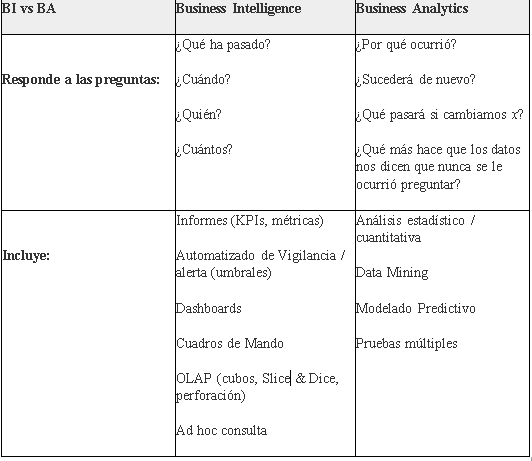
\includegraphics[width=7cm]{./img/img3.png} 
\end{center}

\subsection{ROL DE BUSINESS ANALYTICS Y BUSINESS INTELLIGENCE}
\begin{itemize}
    \item Business Intelligence, es poder desplegar la data de una forma, no precisamente analítica, para que sirva para tomar mejores decisiones.
    \item Business Analytics, ellos son las personas que, en base a la data, pueden saber qué acciones tomar, es decir que pueden realizar un análisis y pueden tomar decisiones.
\end{itemize}

\subsection{CONOCIMIENTOS TÍPICOS SEGÚN EL TIPO DE PERFIL}
\begin{center}
    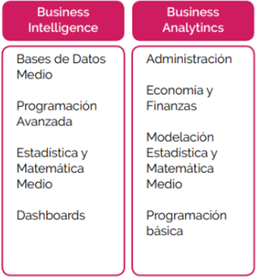
\includegraphics[width=7cm]{./img/img4.png} 
\end{center}

%----------------------------------------------------------------------------------------
%	CONCLUSIONES
%----------------------------------------------------------------------------------------

\section{Conclusiones}
\begin{itemize}	
	\item Las empresas de hoy necesitan herramientas tecnológicas que les permita tomar decisiones de negocio precisas y de forma rápida, ya que los sistemas transaccionales actuales tradicionales, suelen presentar una estructura muy inflexible para este fin.
	\item Las herramientas de BI no vienen a remplazar los sistemas transaccionales actuales, se trata de sistemas con objetivos distintos, eficientes en sus respectivas funciones, pero que deben complementarse para optimizar el valor de los sistemas de información.
	\item BI es una herramienta que se constituye en una ventaja tecnológica ya que con ella se logra centralizar, depurar y afianzar los datos, descubrir información no evidente para las aplicaciones actuales, optimizar el rendimiento de los sistemas.
	\item BI es una herramienta que se constituye en una ventaja competitiva ya que con ella se logra seguimiento real del plan estratégico, aprender de errores pasados, mejorar la competitividad, obtener el verdadero valor de las aplicaciones de gestión.
	\item El mercado ofrece soluciones que son complejas, caras, y presentan importantes deficiencias en cuanto a rendimiento y usabilidad. Por esto se requiere que los proveedores sigan investigando y desarrollando tecnología que mejore la experiencia del usuario.
\end{itemize}

%----------------------------------------------------------------------------------------
%	RECOMENDACIONES
%----------------------------------------------------------------------------------------

\section{Recomendaciones}
Las organizaciones parecen ser conscientes de que el tablero con mejor aspecto no vale nada si los datos mostrados son defectuosos. La inteligencia de negocios no tiene mucho sentido sin una integración completa de datos e iniciativas de calidad de datos, pero éstas deben ser respaldadas con el nivel adecuado de atención, recursos y financiamiento. El respaldo organizativo de la calidad de los datos mediante la implementación de los procesos de propiedad y administración de datos es también vital. La normalización de datos es el trabajo más tedioso y oscuro de la BI, es mejor dedicar las horas a pensar en indicadores que pasarlas en normalizar datos. Por ello es tan importante tener una política de calidad de datos dentro de las empresas. Por ello es necesario diseñar procesos a la hora de realizar el alta de un cliente o de un proveedor.

%----------------------------------------------------------------------------------------
%	BIBLIOGRAFIA
%----------------------------------------------------------------------------------------

\begin{thebibliography}{99} 
    \bibitem{} 
    Almeida, M. S., Ishikawa, M., Reinschmidt, J., \& Roeber, T. (1999). Getting Started with DataWarehouse and Business Intelligence. Recuperado de 
    \\\texttt{http://www.redbooks.ibm.com/redbook\\s/pdfs/sg245415.pdf}
    \bibitem{} 
    Davila, F. (2006). LA INTELIGENCIA DEL NEGOCIO. Recuperado de 
    \\\texttt{http://sigma.poligran.edu.co/polite\\cnico/apoyo/cuadernos/intelligence.pdf}
    \bibitem{} 
    Sinnexus. (2007). Sinnexus. (2007). Business Intelligence. Recuperado de 
    \\\texttt{http://www.sinnexus.com/business\_in\\telligence/index.aspx}
    \bibitem{} 
    Inmon, W. H (1996). Building the data warehouse Jhon Wiley \& Sons Kimball Ralph \& Ross Margy (2002). The Data Warehouse Toolkit: The Complete Guide to Dimensional Modeling. Recuperado de 
    \\\texttt{http://www.sigmod.org/publications\\/sigmodrecord/0309/R17.AnisimovBook\\Review.pdf}
\end{thebibliography}
%----------------------------------------------------------------------------------------
\end{document}